\section{Vytváření podsítí v IPv4}
\label{sec:podsite-ipv4}
Problematika sítí IPv4 je malý počet adres.
Tyto adresy je možné tedy rozdělit na podsítě, které můžeme mít přesně tak velké jak potřebujeme a nemusíme tedy zabírat zbytečně prostor, který bychom mohli využít někde jinde.
Tyto podsítě poté od sebe odlišeujeme stále logickou adresou společně s maskou sítě.
Podsítě v IPv4 se tvoří pomocí dvou způsobů:
\subsection{FLSM - Fixed Length Subnet Mask}
Rozdělení adresného prostoru mezi stejně velké podsítě každou se stejnou maskou.
Využitelné v geograficky omezené oblasti (Velké organizace, univerzity).
Síť s maskou /24, můžeme rozdělit na 2, 4, 8, 16, 32, 64 stejně velkých podsítí.
\subsection{VLSM - Variable Length Subnet Mask}
Rozdělení adresného prostoru mezi podsítě, kde má každá podsíť masku velkou jak je potřeba.
\subsection{Efektivnost technologií}
Efektivnost VLSM bývá mnohem vyšší jelikož je možné vytvořit sítě specificky velké, jak jsou potřeba.
Můžeme se setkat s případy kde by vyřešení podsítí pomocí FLSM nebylo možné i přestože by to pomocí VLSM možné bylo. \\
\subsection{Postup při tvoření podsítí}
\begin{multicols}{2}
  \begin{center}
    Máme IP adresu: \textbf{172.16.32.0/24}
  \end{center}
  \begin{enumerate}
    \item Najdeme největší podsíť. (60)
    \item Pro tuto síť určíme počet bitů potřebných pro umístění všech stanic + 2 pro router a broadcast. (6 bitů pro 62 adres)
    \item Pomocí tohoto vypočítáme masku sítě. (32 - 6 = 26 bitů)
    \item Určíme počet sítí. (4)
    \item Maska podsítě je u FLSM stejná, pro VLSM se mění pro každou podsíť v závislosti na prvních třech krocích.
  \end{enumerate}
  \columnbreak
  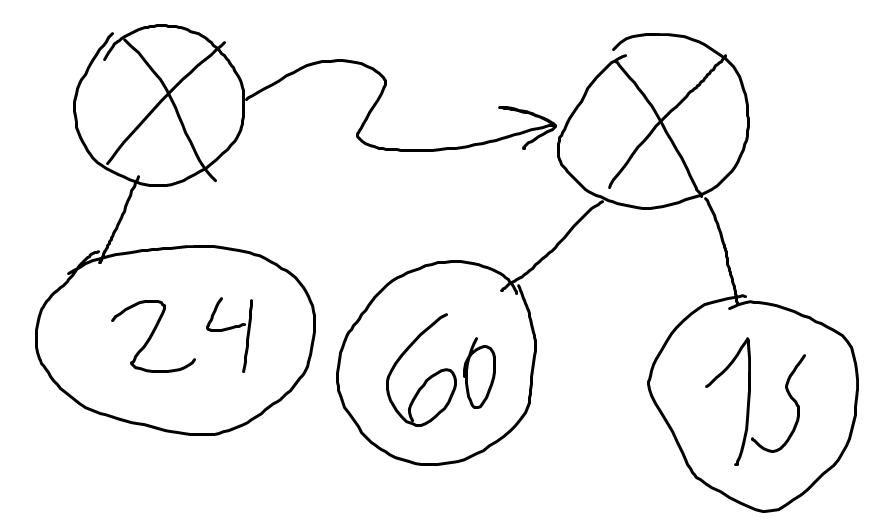
\includegraphics[width=\linewidth]{TVY-POS/Podsite-IPv4/podsit.png}
\end{multicols}
\begin{enumerate}
  \setcounter{enumi}{5}
  \item V posledním bajtu adresy IP zkontrolujeme realizovatelnost podsítí. (2 bity pro 4 masky)
  \item Poté určíme samotné masky podsítí. (00, 01, 10, 11)
  \item Určíme adresy podsítí s maskou. (127.16.32.0/26, 172.16.32.64/26, \dots)
  \item Určíme rozsah adres pro hostitele. (<1;62> 0 je adresa sítě a 63 broadcast)
  \item Podle velikosti určíme pořadí sítí.
  \item Infrastuktury (Routery a switche) sítí budou dostávat nejvyšší možnou adresy v dané podsíti.
  \item Servery dostávají zpravidla nejnižší možnou adresu v dané podsíti.
  \item Zbytek adres se rozdělí pomocí DHCP mezi běžné uživatele.
\end{enumerate}

\[\text{Efektivnost} = \frac{\text{Počet adres využitých}}{\text{Počet adres možných}}\]
